\chapter{Архитектура системы}

\begin{figure}[h]
    \centering
    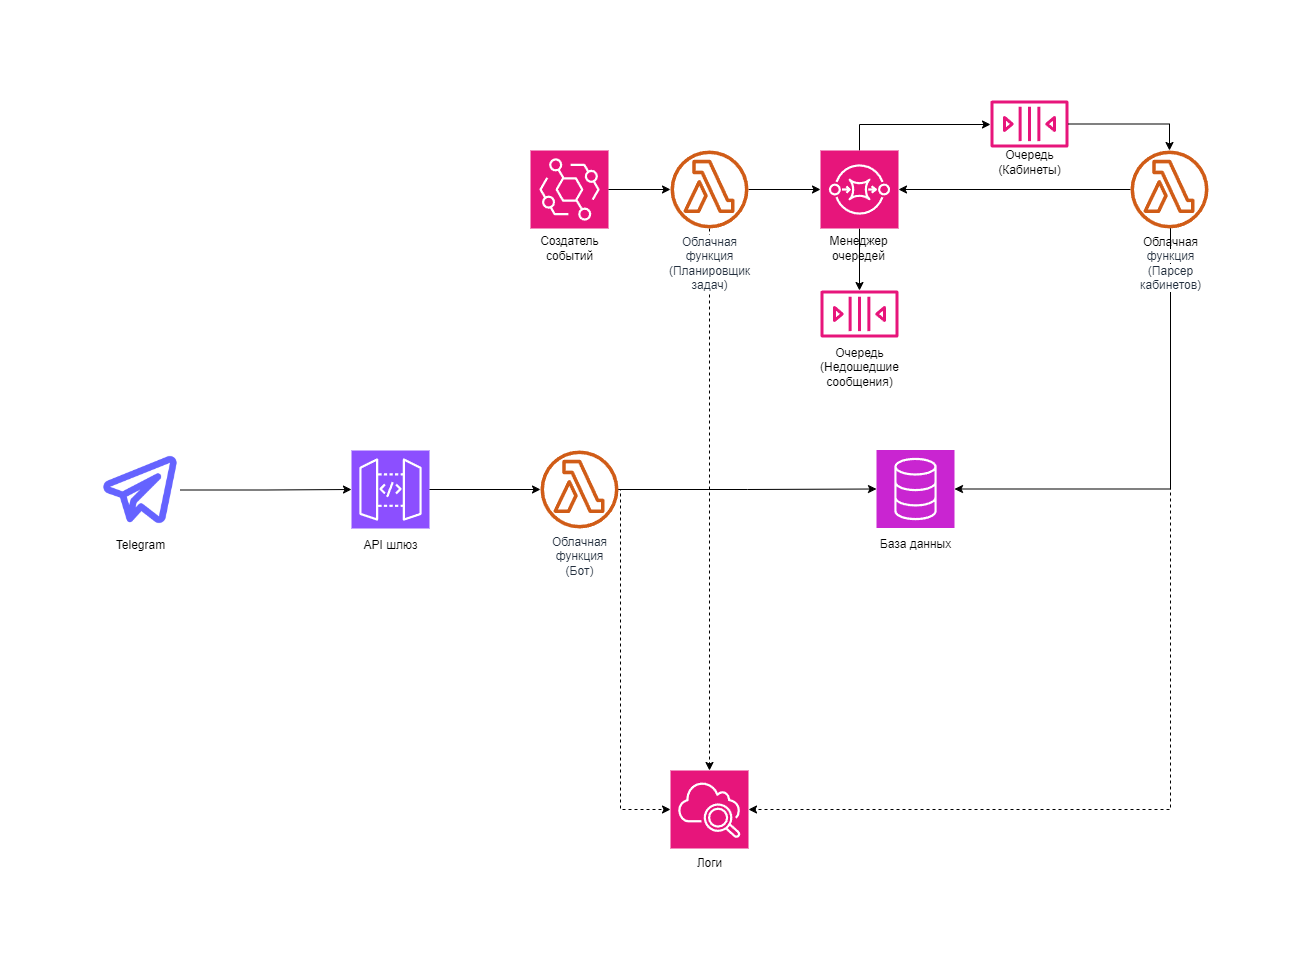
\includegraphics[scale=0.4]{img/functional}
    \caption{Архитектура системы}
    \label{fig:cp}
\end{figure}

\begin{enumerate}
    \item \textbf{Telegram}: Это мессенджер, с которым пользователи
взаимодействуют для отправки и получения сообщений.
    
    \item \textbf{API Шлюз}: Этот компонент обеспечивает взаимодействие между
Telegram и основной функциональностью бота. Он служит мостом для передачи данных
между мессенджером и другими компонентами системы.
    
    \item \textbf{Облачная функция (Бот)}: Центральная часть системы, которая
обрабатывает запросы пользователей и взаимодействует с другими частями системы.
Отсюда отправляются запросы к менеджеру операций, парсеру кабинетов и базе
данных.
    
    \item \textbf{Создатель событий}: Этот компонент генерирует определенные
события или уведомления для менеджера операций.
    
    \item \textbf{Менеджер операций}: Обрабатывает запросы от облачной функции и
координирует выполнение различных операций (выполняет роль автоматического
создателя задач парсеру, т.е какую информацию необходимо собрать с home.mephi).
Также взаимодействует с очередями сообщений.
    
    \item \textbf{Очередь (Кабинеты)}: Хранит информацию о задачах или запросах,
ожидающих выполнения.
    
    \item \textbf{Очередь (Неотвеченные сообщения)}: Хранит информацию о
сообщениях или запросах, на которые еще не был дан ответ в следствие ошибки.
    
    \item \textbf{Облачная функция (Парсер кабинетов)}: Анализирует и
обрабатывает информацию о различных кабинетах с home.mephi.
    
    \item \textbf{База данных}: Хранилище всей информации, необходимой для
работы системы.
    
    \item \textbf{Логи}: Записи о всех операциях и событиях, происходящих в
системе.
\end{enumerate}


\chapter{Выбор модели жизненного цикла}

В контексте рассматриваемого проекта принято решение применять
Agile-методологию. Выбор данной методологии обусловлен следующими причинами:

\begin{enumerate}
    \item \textbf{Динамичность требований.} Agile ориентирован на проекты с
переменчивыми требованиями, что обеспечивает возможность адаптации команды к
обновленным условиям или к обратной связи от стейкхолдеров.
    
    \item \textbf{Оперативная обратная связь.} Основной фокус Agile -- получение
регулярной обратной связи, что способствует раннему обнаружению и решению
проблем, а также проверке соответствия решения ожиданиям заказчика.
    
    \item \textbf{Регулярное обновление продукта.} Agile предполагает частое
внедрение нового функционала, позволяя конечным пользователям активно
тестировать систему и предоставлять свои отзывы.
    
    \item \textbf{Адаптивность.} В условиях переменчивости контекста, как,
например, изменения на web-портале home.mephi, Agile обеспечивает способность
команды к гибкому реагированию.
    
    \item \textbf{Коллаборация.} Agile ставит акцент на совместной работе
разработчиков, заказчика и других участников, создавая прозрачную среду и
атмосферу доверия.
    
    \item \textbf{Ориентированность на пользователя.} В разработке систем с
пользовательским интерфейсом, таких как телеграмм-бот, первостепенное значение
имеет учет требований и потребностей конечного пользователя.
    
    \item \textbf{Мониторинг рисков.} Регулярные итерации и постоянная оценка
позволяют эффективно идентифицировать и контролировать потенциальные риски
проекта.
\end{enumerate}

Учитывая указанные аргументы, применение Agile-методологии для данного проекта
является обоснованным выбором.